\documentclass[11pt, oneside]{article}   	% use "amsart" instead of "article" for AMSLaTeX format
\usepackage{geometry}                		% See geometry.pdf to learn the layout options. There are lots.
\geometry{letterpaper}                   		% ... or a4paper or a5paper or ... 
%\geometry{landscape}                		% Activate for for rotated page geometry
\usepackage[parfill]{parskip}    		% Activate to begin paragraphs with an empty line rather than an indent
\usepackage{graphicx}				% Use pdf, png, jpg, or eps� with pdflatex; use eps in DVI mode
								% TeX will automatically convert eps --> pdf in pdflatex		
\usepackage{amssymb}
\usepackage{amsmath}

\title{Implementation of a Two Grid Formulation in lammpsFOAM}
\author{Rui Sun \and Heng Xiao}
%\date{}							% Activate to display a given date or no date

\begin{document}
\maketitle


\section{Interpolations Needed in a CFD--DEM Solver}
Here, aggregation means Lagrangian phase to Eulerian phase operations; Interpolation means Eulerian phase to Lagrangian phase operations. Sometimes they are also referred to as ``forward'' and ``backward'' interpolations.
\begin{enumerate}
\item  Aggregation of solid volume fraction Eulerian field $\varepsilon_s$ from particle data (position $\mathbf{x}_p$)
\item Aggregation of Eulerian solid-phase velocity $\mathbf{u}_s$ from particle data (position $\mathbf{x}_p$ and velocity $\mathbf{u}_p$)
\item Aggregation of fluid--particle interaction forces onto fluid cells (conservation is essential to ensure momentum balance of the fluid--particle system). See below. 
\item Interpolation of Eulerian fluid-phase velocity field $\mathbf{u}_f$ at particle locations  $\mathbf{u}_{f@p}$ (needed for calculating drag forces); Similar interpolation are needed for $\varepsilon_s$.
\end{enumerate}


\section{Desirable Properties of the Interpolation Procedure}

\begin{enumerate}
\item (Essential) Free of boundary abnormally at both physical boundaries and processor boundaries. For example, for a case with uniformly distributed  particles as in Fig.~\ref{fig:boundary}, the obtained solid volume fraction $\varepsilon_s$ should be a uniform field.
\item  (Essential)  Conservation of mass and momentum, i.e.,
\begin{align} % requires amsmath; align* for no eq. number
\sum_{i = 1}^{N_c} \varepsilon_{s, i} V_{c, i}  & = \sum_{k = 1}^{N_p} V_{p, k}  \\
\sum_{i = 1}^{N_c} \mathbf{F}_{c, i}  & =  -\sum_{k = 1}^{N_p} \mathbf{f}_{p, k}
\end{align}
where $N_c$ is the number of cells in the OpenFOAM mesh; $N_p$ is the number of particles in the system;  $V_{c, i}$ is the  volume of cell $i$; $\mathbf{F}_{c, i}$ is the force on cell $i$ exerted by all particles (in this cell or adjacent cells, depending on the mapping scheme); $\mathbf{f}_{p, k}$ is the force exerted on particle $k$ exerted by the fluid.
\item Convenience of implementation in a parallel code.
\item Convenience of implementation in an unstructured mesh as in OpenFOAM.

\end{enumerate}

\begin{figure}[htbp] %  figure placement: here, top, bottom, or page
   \centering
   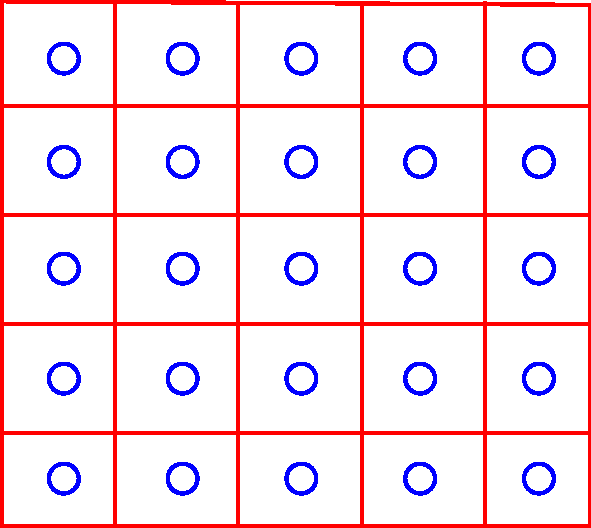
\includegraphics[width=0.4\textwidth]{figs/boundary-abnormal.pdf} 
   \caption{Boundary abnormally requirement.}
   \label{fig:boundary}
\end{figure}


\section{Existing Algorithms and Their Advantages and Drawbacks}

\subsection{Particle Centroid Method} 

\begin{itemize}
\item $+$ satisfies the conservation requirements with straightforward implementation; 
\item + easy implementation on  unstructured mesh;
\item + easy implementation on MPI parallel codes;
\item  $-$ large errors in obtained $\varepsilon_s$ leading to errors in force calculations
\end{itemize}

\subsection{Analytical Method}

\begin{itemize}
\item $+$ better accuracy in obtained $\varepsilon_s$
\item $-$ still would not work if  particle diameter is larger than cell size.
\item $-$ difficulty to implement in unstructured mesh.
\end{itemize}

\subsection{Statistical Kernel Function (Xiao \& Sun)}
\begin{itemize}
\item Difficult and inefficient to implement when bandwidth is larger than 2 or 3 cell width.
\item Better accuracy than PCM, leading to smoother $\varepsilon_s$ field
\end{itemize}

\subsection{Simple Two-Grid Formulation (Deb \& Tafti)}
\begin{itemize}
\item $+$ better accuracy in obtained $\varepsilon_s$ field
\item $+$ Extension to unstructured grid not straightforward
\end{itemize}

\section{Proposed Algorithm}

Calculation solid volume fraction $\varepsilon_s$:
\begin{enumerate}
\item  Construct Cartesian mesh on each processor covering all cells 
on this processor
\item Interpolate all particle volumes to the respective support grid points 
using interpolation function (conservative, Lagrangian to Eulerian)
\item  Compute solid volume fraction at each grid point assuming volume 
as indicated by dashed lines (conservative)
\item  Interpolate the Eulerian volume fraction to OpenFOAM cells 
(Eulerian to Lagrangian not necessarily conservative.  
Need further investigations. Normalize by the ratio of 
volume of Cartesian mesh/volume of OpenFoam.)
\end{enumerate}

\begin{figure}[htbp] 
   \centering
   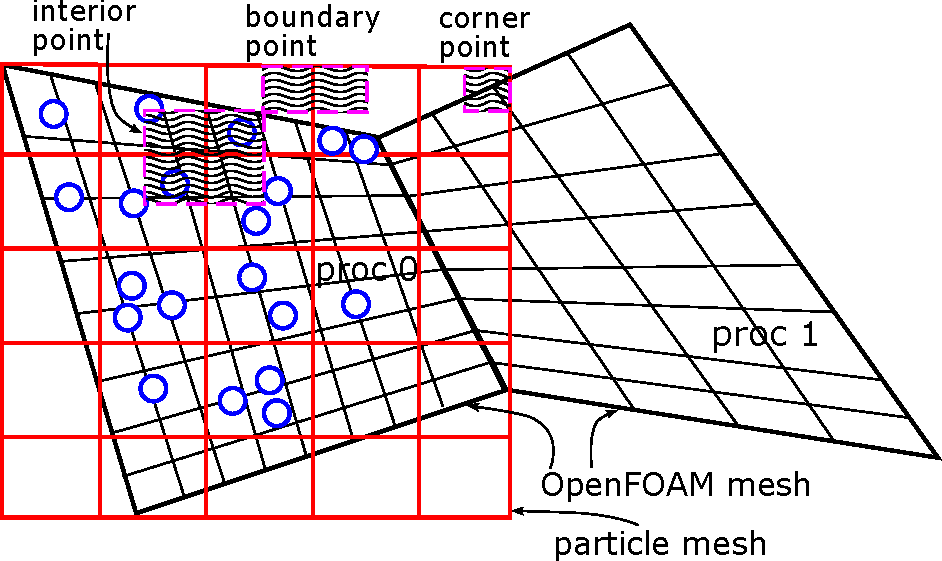
\includegraphics[width=0.85\textwidth]{figs/two-grid} 
   \caption{Proposed two-grid algorithm.}
   \label{fig:two-grid}
\end{figure}

Similar procedure can be followed in calculating the  \emph{Eulerian solid-phase velocity}.
\emph{Interpolation of fluid phase velocity at particle locations}:
No need for such an auxiliary grid. Direct interpolation using the 
procedure in OpenFOAM. 

 Calculation of \emph{particle forces on fluid cells} (conservation is essential)
The strategy is to compute force/volume on each grid point.  (any better methods?)
\begin{enumerate}
\item Compute forces on each particle
\item Map the forces to Cartesian grid points (conservative)
\item Compute force per unit volume on grid points. (conservative)
\item Map force per unit volume onto OpenFOAM cell centers. Renormalize.  
\end{enumerate}


\end{document}  